\section{Second-order processes}\label{sec:2.4}

A photon of \SI{1.2}{eV} carries a momentum of about $\SI{6e-4}{\angstrom^{-1}}$, while the lowest conduction states of silicon sit at a crystal momentum (\cref{sec:1.3}) a large fraction of $2\pi/a = \SI{1.16}{\angstrom^{-1}}$ away from the top of the valence band (\cref{sec:3.3}). The photon has the energy to cross the gap, \SI{1.12}{eV} at \SI{300}{K}, but not the momentum, and the golden rule of \cref{sec:2.1} gives zero. Silicon absorbs such photons all the same, because a lattice vibration can supply the missing momentum. The photon lifts an electron into a state that conserves crystal momentum but not energy, and a phonon emitted or absorbed a moment later takes it to a final state that conserves both. The state in between is never observed. It enters the rate through an energy denominator, the mismatch between its energy and that of the initial state. The treatment follows Refs.~\cite[Chap.~5]{sakurai2017modern} and \cite[Chaps.~I and III]{cohentannoudji1998atom}.

\subsection{Interaction picture and Dyson series}

To go beyond first order we need the amplitude equations \cref{eq:2.1-exact} in a form that iterates, and the interaction picture provides it. Define the state $|\psi_{\mathrm{I}}(t)\rangle = \ee^{\ii H_0t}|\psi(t)\rangle$, whose components are exactly the amplitudes, $c_n(t) = \langle n|\psi_{\mathrm{I}}(t)\rangle$, and the perturbation $H'_{\mathrm{I}}(t) = \ee^{\ii H_0t}H'(t)\,\ee^{-\ii H_0t}$. The Schr\"odinger equation becomes
\begin{equation}
  \ii\,\partial_t|\psi_{\mathrm{I}}(t)\rangle = H'_{\mathrm{I}}(t)\,|\psi_{\mathrm{I}}(t)\rangle ,
  \label{eq:2.4-ipicture}
\end{equation}
whose matrix elements in the basis $|n\rangle$ are \cref{eq:2.1-exact}. The free evolution sits in the operator: $\langle m|H'_{\mathrm{I}}(t)|n\rangle = H'_{mn}(t)\,\ee^{\ii(E_m - E_n)t}$, with $H'_{mn}(t) \equiv \langle m|H'(t)|n\rangle$. For independent electrons this is the oscillation $\ee^{\ii(E_\gamma - E_{\gamma'})t}$ of $c^\dagger_\gamma c_{\gamma'}$ found in \cref{sec:2.3}.

Integrating \cref{eq:2.4-ipicture} from $t_0$ to $t$ and inserting the result into its own right-hand side, again and again, leads to the evolution operator of the interaction picture as a power series in $H'$, the Dyson series,
\begin{equation}
  U_{\mathrm{I}}(t, t_0) = 1 - \ii\int_{t_0}^{t}\dd t_1\,H'_{\mathrm{I}}(t_1) + (-\ii)^2\int_{t_0}^{t}\dd t_1\int_{t_0}^{t_1}\dd t_2\,H'_{\mathrm{I}}(t_1)\,H'_{\mathrm{I}}(t_2) + \dots ,
  \label{eq:2.4-dyson}
\end{equation}
with $|\psi_{\mathrm{I}}(t)\rangle = U_{\mathrm{I}}(t, t_0)|\psi_{\mathrm{I}}(t_0)\rangle$. In each term the operators stand in order of decreasing time from left to right, which is why the series is also called the time-ordered exponential of $-\ii\int H'_{\mathrm{I}}$. The first-order term reproduces \cref{eq:2.1-c1}. A complete set of states $|m\rangle$ between the two factors of the second-order term leads to the amplitude for $f \ne i$,
\begin{equation}
  c^{(2)}_f(t) = (-\ii)^2\sum_m\int_{t_0}^{t}\dd t_1\int_{t_0}^{t_1}\dd t_2\;H'_{fm}(t_1)\,\ee^{\ii(E_f - E_m)t_1}\;H'_{mi}(t_2)\,\ee^{\ii(E_m - E_i)t_2} .
  \label{eq:2.4-c2}
\end{equation}
It reads from right to left as a story: at $t_2$ the perturbation takes the system from $i$ to $m$, it evolves freely in $m$ until $t_1$, and at $t_1$ the perturbation takes it to $f$. Every state $m$ contributes, $m = i$ and $m = f$ included, and the amplitudes of the different $m$ add. Each further order adds one more factor of $H'$ and one more time integral. For a constant perturbation acting for a time $t$, the terms of \cref{eq:2.4-dyson} grow as powers of $|H'|t$, the expansion parameter of \cref{sec:2.1}. Once the time integrals are done in the long-time limit, the powers of $t$ turn into powers of $|H'|$ divided by energy differences.

\subsection{Second-order golden rule}

For a constant perturbation the time integrals in \cref{eq:2.4-c2} are elementary once we decide how $H'$ is switched on. \Cref{sec:2.1} showed that a rate does not depend on the switching. The most convenient choice is to turn $H'$ on slowly in the remote past, $H'(t) = H'\,\ee^{t/\tau_{\mathrm{s}}}$ with $t_0 \to -\infty$, and to let the switching time $\tau_{\mathrm{s}}$ go to infinity at the end, at fixed $t$. The inner integral is then
\begin{equation*}
  \int_{-\infty}^{t_1}\dd t_2\,\ee^{[\ii(E_m - E_i) + 1/\tau_{\mathrm{s}}]t_2}
  = \frac{\ii\,\ee^{[\ii(E_m - E_i) + 1/\tau_{\mathrm{s}}]t_1}}{E_i - E_m + \ii/\tau_{\mathrm{s}}} .
\end{equation*}
The free phase that the system accumulates in $m$ has turned into a factor $1/(E_i - E_m)$, the \emph{energy denominator}, and the switching has put a small positive imaginary part into it. The rest of the integrand of \cref{eq:2.4-c2} has the form of the first-order one, with $\xi = E_f - E_i$ and the switching rate doubled. The amplitude to second order is
\begin{equation*}
  c_f(t) = -\ee^{\ii\xi t}\left[\frac{A_1\,\ee^{t/\tau_{\mathrm{s}}}}{\xi - \ii/\tau_{\mathrm{s}}} + \frac{A_2\,\ee^{2t/\tau_{\mathrm{s}}}}{\xi - 2\ii/\tau_{\mathrm{s}}}\right],
  \qquad A_1 = H'_{fi},\quad A_2 = \sum_m\frac{H'_{fm}H'_{mi}}{E_i - E_m + \ii0^+} ,
\end{equation*}
where $\ii0^+$ stands for $\ii/\tau_{\mathrm{s}}$ in the limit. The transition rate is the time derivative of $|c_f|^2$. The squared first-order term contributes $(2/\tau_{\mathrm{s}})\,\ee^{2t/\tau_{\mathrm{s}}}|A_1|^2/(\xi^2 + 1/\tau_{\mathrm{s}}^2)$, a Lorentzian of area $2\pi|A_1|^2$ whose width vanishes with $1/\tau_{\mathrm{s}}$, and it tends to $2\pi|A_1|^2\delta(\xi)$; the squared second-order term does the same with $2/\tau_{\mathrm{s}}$ in place of $1/\tau_{\mathrm{s}}$. The cross term needs more care, since the two terms carry different switching rates. Its derivative is
\begin{equation*}
  2\Real\!\left[A_1A_2^*\,\ee^{3t/\tau_{\mathrm{s}}}\,\frac{3/\tau_{\mathrm{s}}}{(\xi - \ii/\tau_{\mathrm{s}})(\xi + 2\ii/\tau_{\mathrm{s}})}\right] .
\end{equation*}
The fraction falls off as $1/\xi^2$, and its only pole in the upper half plane is at $\xi = \ii/\tau_{\mathrm{s}}$. Closing the contour there, the integral over $\xi$ is $2\pi\ii\,(3/\tau_{\mathrm{s}})/(3\ii/\tau_{\mathrm{s}}) = 2\pi$, independent of $\tau_{\mathrm{s}}$, while its width shrinks as $1/\tau_{\mathrm{s}}$. Its imaginary part is odd in $\xi$ and drops out against any smooth function. The cross term therefore tends to $2\pi\cdot 2\Real(A_1A_2^*)\,\delta(\xi)$. The three terms combine into a single squared modulus:
\begin{keyresult}[Second-order golden rule]
\begin{equation}
  \varGamma_{i\to f} = 2\pi\,|T_{fi}|^2\,\delta(E_f - E_i), \qquad
  T_{fi} = H'_{fi} + \sum_m\frac{H'_{fm}\,H'_{mi}}{E_i - E_m + \ii0^+} + \dots .
  \label{eq:2.4-golden2}
\end{equation}
The sum runs over all intermediate states $m$; the rate is defined after summation over a continuum of final states, as in \cref{eq:2.1-golden}.
\end{keyresult}

The quantity $T_{fi}$ is the element of the transition matrix, or T-matrix. Continued to all orders, the Dyson series becomes a geometric series in the energy denominators, which sums to the Lippmann--Schwinger equation~\cite[Chap.~6]{sakurai2017modern}
\begin{equation}
  T_{fi} = H'_{fi} + \sum_m\frac{H'_{fm}\,T_{mi}}{E_i - E_m + \ii0^+} .
  \label{eq:2.4-LS}
\end{equation}
Iterating it once reproduces \cref{eq:2.4-golden2}. In the language of \cref{sec:2.1}, the S-matrix element is $\delta_{fi} - 2\pi\ii\,\delta(E_f - E_i)\,T_{fi}$, and $T_{fi}$ equals the invariant amplitude $-\mathcal{M}$ divided by the normalization factors of the box matrix element of \cref{sec:2.1}, at every order.

Energy is conserved between the initial and the final state, through $\delta(E_f - E_i)$, but not in the intermediate state: $E_m$ can be anything. The intermediate state is \emph{virtual}. The phase $\ee^{\ii(E_m - E_i)t_2}$ in \cref{eq:2.4-c2} oscillates with period $2\pi/|E_i - E_m|$, and contributions from times $t_2$ further than about $1/|E_i - E_m|$ before $t_1$ cancel. The system spends a time of that size in $m$. The further $m$ is from the initial energy, the shorter the time and the smaller the amplitude. The physical content is the energy--time relation. A state $m$ with $E_m = E_i$ is \emph{on shell}, any other one \emph{off shell}, and an on-shell intermediate state makes the denominator vanish.

The second-order term is small compared to the first by a factor $\sim|H'_{fm}|/|E_i - E_m|$, the coupling measured against the energy mismatch. For dark-matter scattering this factor is the Born parameter of \cref{sec:2.2}. The second-order term of \cref{eq:2.4-golden2}, with plane-wave intermediate states, is the second Born term, and it is suppressed by $y_\chi y_e\,\mu_{\chi e}/(4\pi m_V)$ or $y_\chi y_e/(4\pi v)$, numbers below $10^{-3}$ for the couplings that are still allowed. Second-order processes matter in this book for another reason: when first order is closed, an internal interaction of the target, such as the coupling of electrons to phonons, can open the channel.

Classical fields fit the same formula. If $H'$ contains harmonic terms $\op{O}_j\ee^{-\ii\omega_jt}$, as in \cref{sec:2.1}, each factor $H'_{\mathrm{I}}$ in \cref{eq:2.4-c2} carries its own frequency. The inner time integral then produces the denominator $E_i + \omega_j - E_m$ for the field $j$ that acts first. The outer one leads to $\delta(E_f - E_i - \omega_j - \omega_k)$ in the rate, with $\omega_k$ the frequency of the field that acts second. An emission term enters with $-\omega$ in place of $\omega$. The result is the same as if each field were a quantized mode whose photon energy is part of $E_i$, $E_m$ and $E_f$, and we use whichever language is clearer.

The second-order golden rule also inherits the time window of \cref{eq:2.1-window}, with one more condition. The energy denominator replaces the free phase in $m$ only after that phase has oscillated many times, and the derivation took $\tau_{\mathrm{s}} \to \infty$ to ensure this. As long as we watch for longer than $1/|E_i - E_m|$, about a femtosecond below a direct gap of a few eV, the denominator form holds, and every measurement satisfies this. Near a resonance the condition fails, and it is replaced by $t \gg 1/\varGamma_{\mathrm{w}}$, where $\varGamma_{\mathrm{w}}$ is the decay width of the real intermediate state (\cref{eq:2.4-width}).

\subsection{Time orderings}

The phonon-assisted absorption of the opening paragraph has the general structure of a second-order process in which a target absorbs one quantum and emits another. Let quantum 1, of energy $\omega_1$, be absorbed, and quantum 2, of energy $\omega_2$, be emitted, while the target goes from a state $|i_{\mathrm{T}}\rangle$ to a state $|f_{\mathrm{T}}\rangle$, with the subscript T for target. In the language of \cref{sec:2.3} the two quanta are boson modes with operators $d_1$ and $d_2$, and the perturbation is a sum of two terms that each change one occupation by one,
\begin{equation*}
  H' = H_1 + H_2, \qquad H_1 = \op{O}_a\,d_1 + \op{O}_a^\dagger\,d_1^\dagger, \qquad H_2 = \op{O}_b\,d_2 + \op{O}_b^\dagger\,d_2^\dagger ,
\end{equation*}
with $\op{O}_a$ and $\op{O}_b$ operators on the target. The initial state $|i\rangle = |i_{\mathrm{T}};\,n_1 = 1, n_2 = 0\rangle$ has energy $E_i = E_{i_{\mathrm{T}}} + \omega_1$, and the final state $|f\rangle = |f_{\mathrm{T}};\,0, 1\rangle$ has $E_f = E_{f_{\mathrm{T}}} + \omega_2$. Neither $H_1$ nor $H_2$ connects them, since each changes only one occupation, and $H'_{fi} = 0$. At second order there are two routes, drawn in \cref{fig:2-orderings}. In the absorb-first ordering, $H_1$ acts first and removes quantum 1; the intermediate state $|m;\,0, 0\rangle$ has energy $E_m$. In the emit-first ordering, $H_2$ acts first and creates quantum 2 while quantum 1 is still present; the intermediate state $|m;\,1, 1\rangle$ has energy $E_m + \omega_1 + \omega_2$. Inserting both into \cref{eq:2.4-golden2}, with $d_1|1\rangle = |0\rangle$ and $d_2^\dagger|0\rangle = |1\rangle$,
\begin{equation}
  T_{fi} = \sum_m\left[\frac{\langle f_{\mathrm{T}}|\op{O}_b^\dagger|m\rangle\langle m|\op{O}_a|i_{\mathrm{T}}\rangle}{E_{i_{\mathrm{T}}} + \omega_1 - E_m + \ii0^+}
  + \frac{\langle f_{\mathrm{T}}|\op{O}_a|m\rangle\langle m|\op{O}_b^\dagger|i_{\mathrm{T}}\rangle}{E_{i_{\mathrm{T}}} - \omega_2 - E_m + \ii0^+}\right],
  \label{eq:2.4-orderings}
\end{equation}
and energy conservation, $E_{f_{\mathrm{T}}} + \omega_2 = E_{i_{\mathrm{T}}} + \omega_1$, holds between $i$ and $f$ but not in between.

\begin{figure}[tbp]
  \centering
  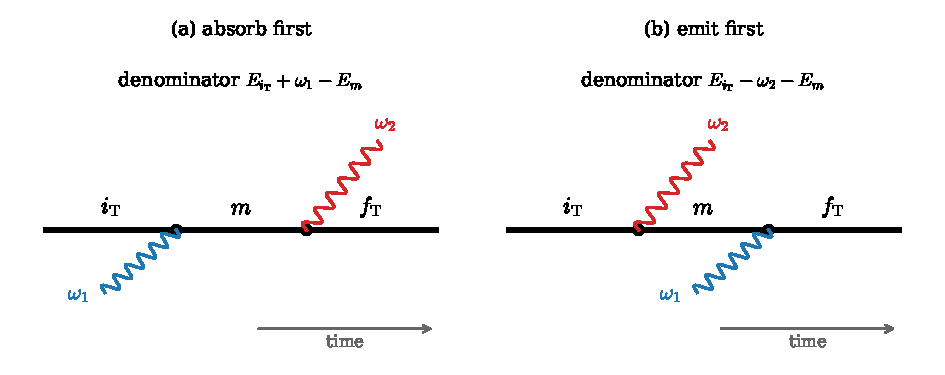
\includegraphics[width=\linewidth]{figures/ch02/fig2_4.pdf}
  \caption{The two time orderings of a second-order process in which a target goes from state $i_{\mathrm{T}}$ to state $f_{\mathrm{T}}$ while absorbing a quantum of energy $\omega_1$ and emitting one of energy $\omega_2$. Time runs to the right; the thick line is the target and the wavy lines are the quanta (absorbed from below, emitted upward). (a) Absorb first: the intermediate state is the target in $m$ with no quanta, of energy $E_m$. (b) Emit first: the target is in $m$ while both quanta are present, of energy $E_m + \omega_1 + \omega_2$. Each panel gives the energy denominator, the initial energy $E_{i_{\mathrm{T}}} + \omega_1$ minus the intermediate energy, with which its amplitude enters \cref{eq:2.4-orderings}.}
  \label{fig:2-orderings}
\end{figure}

Both orderings connect the same states, and their amplitudes add before squaring and can interfere. If $i_{\mathrm{T}}$ is the ground state of the target, $E_m \ge E_{i_{\mathrm{T}}}$ for every $m$, and the emit-first denominator $E_{i_{\mathrm{T}}} - \omega_2 - E_m$ is at most $-\omega_2$: it never vanishes, and this ordering is always off shell. The absorb-first denominator vanishes when $\omega_1 = E_m - E_{i_{\mathrm{T}}}$, that is, when quantum 1 alone could excite the target to a real state $m$. This is the resonance, and near it the absorb-first ordering dominates. Far from every resonance the two orderings are of similar size, and dropping one changes the rate by a factor of a few or more, as \cref{we:2-twophoton} shows. In silicon, with quantum 1 a photon and quantum 2 a phonon, \cref{eq:2.4-orderings} is the bracket of the theory of phonon-assisted absorption of Hall, Bardeen and Blatt~\cite{hall1954infrared}, which also includes phonon absorption in place of emission; Ref.~\cite[Eq.~(200)]{giustino2017electron} writes it in first-principles form. The photon-first term has the denominator of a direct, vertical transition at fixed crystal momentum, and the phonon-first term the denominator of an electron scattered by the phonon before the photon arrives. \Cref{sec:6.5} evaluates both. When the modes hold $n_1$ and $n_2$ quanta rather than one and zero, the matrix elements of $d_1$ and $d_2^\dagger$ bring factors $\sqrt{n_1}$ and $\sqrt{n_2 + 1}$, in both orderings alike; \cref{sec:2.5} averages them over thermal populations.

In a target with many electrons, $i_{\mathrm{T}}$, $m$ and $f_{\mathrm{T}}$ are the many-electron states of \cref{sec:2.3}, and the denominators are differences of total energies. For independent electrons they reduce to differences of orbital energies, because an operator that moves one electron from $\gamma'$ to $\gamma$ changes the total energy by $E_\gamma - E_{\gamma'}$, the frequency at which $c^\dagger_\gamma c_{\gamma'}$ oscillates in the interaction picture. If the photon moves an electron from an occupied valence orbital to an empty conduction orbital at the same crystal momentum, the absorb-first denominator is the photon energy minus that vertical transition energy, whatever the other electrons do. The Pauli principle changes the list of intermediate states. A state in which the moved electron would enter an occupied orbital does not exist. In its place there are orderings in which a different electron moves first and the electron moved by the photon then fills the hole it left, with the anticommutation sign of \cref{sec:2.3} attached to the amplitude. The single-particle picture of one electron passing through an intermediate band is a convenient way of organizing these terms, not a literal history, and \cref{sec:6.5} counts them for silicon.

\subsection{Resonance and finite width}

At resonance the absorb-first term of \cref{eq:2.4-orderings} is infinite, and the rate with it. Nothing in nature diverges here. The trouble is that \cref{eq:2.4-c2} lets the system stay in $m$ forever with unit probability, while a real excited state decays. Quantum 1 can take the target to $m$, and $m$ then empties into $f_{\mathrm{T}}$ by emitting quantum 2, or into any other state it is coupled to. We need the time dependence of a state that decays into a continuum, and this is the Wigner--Weisskopf problem~\cite{weisskopf1930berechnung}. A state that empties at rate $\varGamma_{\mathrm{w}}$ survives for a time of about $1/\varGamma_{\mathrm{w}}$, so its energy is defined only to within about $\varGamma_{\mathrm{w}}$, and a denominator that would vanish should instead saturate at a size of order $\varGamma_{\mathrm{w}}$.

Take a discrete state $|i\rangle$ coupled by a constant $H'$ to a continuum of states $|f\rangle$, with no other couplings, as in \cref{sec:2.1}. \Cref{app:D.3} solves the amplitude equations \cref{eq:2.1-exact} for this case without assuming that $c_i$ stays close to one. Under the condition that made the golden rule possible, $\varGamma_i \ll E_{\mathrm{w}}$, the memory of the continuum is short compared with the decay time. At times $t \gg 1/E_{\mathrm{w}}$ the amplitude of the initial state is then
\begin{equation}
  c_i(t) = \ee^{-(\varGamma_i/2 + \ii\Delta E_i)\,t}, \qquad
  \Delta E_i = \operatorname{PV}\sum_f\frac{|H'_{fi}|^2}{E_i - E_f} ,
  \label{eq:2.4-WW}
\end{equation}
where $\varGamma_i$ is the golden-rule rate \cref{eq:2.1-total} and $\operatorname{PV}$ denotes the principal value of the sum, made precise in the next subsection. The probability $|c_i|^2 = \ee^{-\varGamma_it}$ decays exponentially at the golden-rule rate, which justifies the statement of \cref{sec:2.1} that $\varGamma_i$ keeps its meaning beyond the first-order window (\cref{we:2-continuum}). The energy of the state is shifted by $\Delta E_i$, the second-order level shift of stationary perturbation theory, now with the principal value that a continuum requires; in \cref{we:2-continuum} the shift vanishes because the continuum is symmetric about resonance. The populations of the final states at late times trace out the line,
\begin{equation}
  |c_f(\infty)|^2 = \frac{|H'_{fi}|^2}{(E_f - E_i - \Delta E_i)^2 + \varGamma_i^2/4} ,
  \label{eq:2.4-lorentz}
\end{equation}
a Lorentzian of full width $\varGamma_i$ at half maximum, centered at the shifted energy. Summed over the continuum with density $\mathcal{D}_f$, it integrates to $\overline{|H'_{fi}|^2}\mathcal{D}_f\cdot 2\pi/\varGamma_i = 1$: the decaying state has gone somewhere, and the golden-rule rate fixes both how fast and how sharply in energy. The same shape describes the cross-section near a resonance in scattering, where it is called a Breit--Wigner line. \Cref{app:D.3} also states the limits of the exponential law. It fails at times shorter than $1/E_{\mathrm{w}}$, where the decay starts quadratically as in \cref{we:2-continuum}. It also fails after many lifetimes, where the edges of the continuum leave a slow power-law tail, by then far below any measurable level when $\varGamma_i \ll E_{\mathrm{w}}$.

Back to the intermediate state. Between $t_2$ and $t_1$ in \cref{eq:2.4-c2} the system evolves in $m$. \Cref{eq:2.4-WW} applied to $m$ replaces its free phase $\ee^{-\ii E_m(t_1 - t_2)}$ by $\ee^{-\ii(\tilde E_m - \ii\varGamma_{\mathrm{w}}/2)(t_1 - t_2)}$, where $\tilde E_m = E_m + \Delta E_m$ is the shifted energy and $\varGamma_{\mathrm{w}}$ the total decay rate of $m$, summed over all of its decay channels. The inner time integral then converges without any switching and gives
\begin{equation}
  \frac{1}{E_i - E_m + \ii0^+} \;\longrightarrow\; \frac{1}{E_i - \tilde E_m + \ii\varGamma_{\mathrm{w}}/2} .
  \label{eq:2.4-width}
\end{equation}
The infinitesimal becomes a finite width, and at resonance the amplitude is large, $-2\ii/\varGamma_{\mathrm{w}}$ in place of the denominator, but finite. In the language of the Dyson series, \cref{eq:2.4-width} keeps, from every order, the repeated emission and reabsorption that happen while the system sits in $m$. These are the terms that grow near resonance, and summing them is consistent under the same condition as before, $\varGamma_{\mathrm{w}}$ small compared with the energy over which the decay continuum of $m$ changes. Off resonance, with $|E_i - \tilde E_m| \gg \varGamma_{\mathrm{w}}$, the width is a small correction and the shift is usually absorbed in the measured energy $\tilde E_m$. From now on we write $E_m$ for the shifted energy. In a solid the width of an excited electron comes from the emission of phonons and from scattering with other electrons, and it depends on how far above the band edge the electron sits; \cref{sec:6.3} computes the phonon part. For the off-resonant denominators that dominate below a direct gap, an infinitesimal $\ii0^+$ is enough.

\subsection{Principal value and finite part}

An energy denominator regularized by a width, $1/(x + \ii\varGamma_{\mathrm{w}}/2)$ with $x = E_i - E_m$, has a real and an imaginary part,
\begin{equation*}
  \frac{1}{x + \ii\varGamma_{\mathrm{w}}/2} = \frac{x}{x^2 + \varGamma_{\mathrm{w}}^2/4} - \ii\,\frac{\varGamma_{\mathrm{w}}/2}{x^2 + \varGamma_{\mathrm{w}}^2/4} ,
\end{equation*}
drawn in \cref{fig:2-denominator}(a). The real part equals $1/x$ for $|x| \gg \varGamma_{\mathrm{w}}$ and turns over smoothly through zero inside $|x| < \varGamma_{\mathrm{w}}/2$, with extrema $\pm1/\varGamma_{\mathrm{w}}$. The imaginary part is a Lorentzian of area $\pi$ and depth $2/\varGamma_{\mathrm{w}}$. As $\varGamma_{\mathrm{w}} \to 0$ the Lorentzian becomes $\pi\delta(x)$. The real part, integrated against a smooth function $w(x)$, becomes $\int\dd x\,x[w(x) - w(0)]/(x^2 + \varGamma_{\mathrm{w}}^2/4)$, since $x/(x^2 + \varGamma_{\mathrm{w}}^2/4)$ is odd, and this tends to $\int\dd x\,[w(x) - w(0)]/x$. That is the principal value of $\int\dd x\,w(x)/x$: the integral with a symmetric interval $(-x_{\mathrm{c}}, x_{\mathrm{c}})$ cut out around the pole, in the limit $x_{\mathrm{c}} \to 0$, in which the divergences on the two sides cancel. Together these limits are the Sokhotski--Plemelj formula,
\begin{equation}
  \frac{1}{x + \ii0^+} = \operatorname{PV}\frac{1}{x} - \ii\pi\,\delta(x) ,
  \label{eq:2.4-SP}
\end{equation}
which \cref{app:C.4} proves for the general case. Applied to a second-order amplitude, it splits the sum over intermediate states into two parts with different physics. The principal-value part collects the off-shell intermediate states, and it is real: it shifts energies, as $\Delta E_i$ does in \cref{eq:2.4-WW}, and it produces the dispersive effects of a medium. The delta part picks out the on-shell intermediate states, those with $E_m = E_i$; it is imaginary and produces the decay. \Cref{eq:2.4-WW} is the example: the self-coupling of $i$ through the continuum, $\sum_f|H'_{fi}|^2/(E_i - E_f + \ii0^+)$, is $\Delta E_i - \ii\varGamma_i/2$ by \cref{eq:2.4-SP}. The same statement can be read off the T-matrix. The forward element at second order, $T_{ii} = \sum_f|H'_{fi}|^2/(E_i - E_f + \ii0^+)$, has imaginary part $-\pi\sum_f|H'_{fi}|^2\delta(E_f - E_i) = -\varGamma_i/2$. The total decay rate of a state is $-2\Imag T_{ii}$, the lowest-order form of the optical theorem, which follows in general from the unitarity of the evolution: the probability that leaves $i$ is the probability that arrives in all the states $f$.

The principal-value part has a familiar instance in light scattering. Let quanta 1 and 2 be photons of the same frequency, so that the target absorbs one photon and emits another and returns to $f_{\mathrm{T}} = i_{\mathrm{T}}$. \Cref{eq:2.4-orderings} is then the amplitude of elastic (Rayleigh) scattering, and below every resonance both orderings are off shell and real. Summed over intermediate states, the two orderings combine into $\sum_m 2(E_m - E_{i_{\mathrm{T}}})|\langle m|\op{O}|i_{\mathrm{T}}\rangle|^2/[\omega^2 - (E_m - E_{i_{\mathrm{T}}})^2]$, for a Hermitian $\op{O}$. For a dipole coupling, $\op{O}$ is the field amplitude times the dipole operator along the field, and the sum is minus the dynamic polarizability of the target, whose denominators are $(E_m - E_{i_{\mathrm{T}}})^2 - \omega^2$, times the square of the field amplitude. Its imaginary part, which appears once a width or a continuum puts the absorb-first denominator on shell, is absorption. The dielectric function of \cref{sec:4.4} has the same structure, with a real part made of off-shell transitions and an imaginary part made of on-shell ones.

\begin{figure}[tbp]
  \centering
  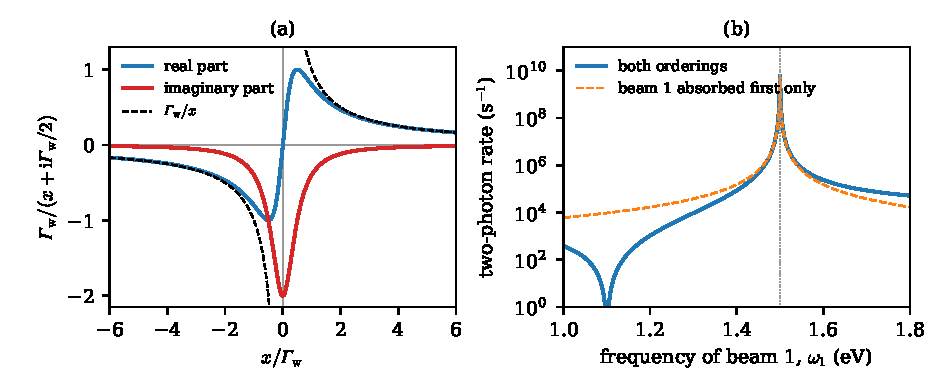
\includegraphics[width=\linewidth]{figures/ch02/fig2_5.pdf}
  \caption{(a) Real and imaginary parts of an energy denominator regularized by a width, $1/(x + \ii\varGamma_{\mathrm{w}}/2)$, multiplied by $\varGamma_{\mathrm{w}}$ and plotted against $x/\varGamma_{\mathrm{w}}$, where $x$ is the initial energy minus the intermediate energy. Dashed: $\varGamma_{\mathrm{w}}/x$, to which the real part tends for $|x| \gg \varGamma_{\mathrm{w}}$. As $\varGamma_{\mathrm{w}} \to 0$ the real part becomes the principal value of $1/x$ and the imaginary part $-\pi\delta(x)$. (b) Rate of two-photon absorption in the three-level model of \cref{we:2-twophoton}, against the frequency $\omega_1$ of beam 1 at fixed $\omega_2 = \SI{1.90}{eV}$, for the channel with final energy $\omega_1 + \omega_2$. The model has a ground level $i_{\mathrm{T}}$, an intermediate level $m$ at \SI{1.50}{eV} with total width $\varGamma_{\mathrm{w}} = \SI{1}{meV}$, and a flat band of final states above \SI{3.20}{eV}. Either beam drives $i_{\mathrm{T}} \to m$ with matrix element \SI{0.1}{meV}, and beam 2 empties a real level $m$ into the band at the rate \SI{0.1}{meV}. Solid: both time orderings. Dashed: the ordering in which beam 1 is absorbed first, alone. The peak at $\omega_1 = \SI{1.50}{eV}$ is the resonance with $m$; the zero at \SI{1.10}{eV} is destructive interference between the two orderings.}
  \label{fig:2-denominator}
\end{figure}

The rate needs the squared modulus, and near resonance this brings a double pole. With $|E_i - E_m + \ii\varGamma_{\mathrm{w}}/2|^{-2} = 1/(x^2 + \varGamma_{\mathrm{w}}^2/4)$, the limit $\varGamma_{\mathrm{w}} \to 0$ cannot be taken in \cref{eq:2.4-SP}: the square of $\ii\pi\delta(x)$ has no meaning, as the square of the momentum delta function had none in \cref{sec:2.1}. The function $1/x^2$ has no principal value either. Its singularity is even, the divergences on the two sides add instead of cancelling, and $\int_{|x| > x_{\mathrm{c}}}\dd x/x^2 = 2/x_{\mathrm{c}}$. The Hadamard finite part removes exactly this divergence:
\begin{equation}
  \operatorname{fp}\!\int\dd x\,\frac{w(x)}{x^2}
  = \lim_{x_{\mathrm{c}}\to0}\left[\int_{|x|>x_{\mathrm{c}}}\dd x\,\frac{w(x)}{x^2} - \frac{2w(0)}{x_{\mathrm{c}}}\right]
  = \int_0^\infty\dd x\,\frac{w(x) + w(-x) - 2w(0)}{x^2} .
  \label{eq:2.4-fp}
\end{equation}
The integrand on the right is finite at $x = 0$, where it tends to $w''(0)$. With it, the Lorentzian of the rate splits as follows. Write $\int\dd x\,w(x)/(x^2 + \varGamma_{\mathrm{w}}^2/4)$ as $w(0)\int\dd x/(x^2 + \varGamma_{\mathrm{w}}^2/4) = 2\pi w(0)/\varGamma_{\mathrm{w}}$ plus $\int\dd x\,[w(x) - w(0)]/(x^2 + \varGamma_{\mathrm{w}}^2/4)$. The remainder tends to the finite part as $\varGamma_{\mathrm{w}} \to 0$, since its integrand is integrable at $x = 0$. Its difference from the limit is $-(\varGamma_{\mathrm{w}}^2/4)\int\dd x\,[w(x) - w(0)]/[x^2(x^2 + \varGamma_{\mathrm{w}}^2/4)]$, which is dominated by $|x| \lesssim \varGamma_{\mathrm{w}}$. There the odd part of $w(x) - w(0)$ drops out and the even part is $w''(0)x^2/2$, and the difference is $-(\varGamma_{\mathrm{w}}^2/8)\,w''(0)\cdot 2\pi/\varGamma_{\mathrm{w}} = -\pi\varGamma_{\mathrm{w}}w''(0)/4$. In the sense of distributions,
\begin{equation}
  \frac{1}{x^2 + \varGamma_{\mathrm{w}}^2/4} = \frac{2\pi}{\varGamma_{\mathrm{w}}}\,\delta(x) + \operatorname{fp}\frac{1}{x^2} - \frac{\pi\varGamma_{\mathrm{w}}}{4}\,\delta''(x) + O(\varGamma_{\mathrm{w}}^2) .
  \label{eq:2.4-split}
\end{equation}
For a function $w$ that varies on an energy scale $\Delta_{\mathrm{w}}$, the delta term is of size $w/\varGamma_{\mathrm{w}}$, the finite part of size $w/\Delta_{\mathrm{w}}$, and the correction a fraction $(\varGamma_{\mathrm{w}}/\Delta_{\mathrm{w}})^2$ of the delta term. \Cref{app:C.4} collects these definitions.

The two terms of \cref{eq:2.4-split} are the on-shell and the off-shell parts of a resonant second-order rate, and the on-shell part has a direct interpretation. Inserted in \cref{eq:2.4-golden2}, the delta term of the absorb-first ordering is the first-order golden-rule rate $2\pi|\langle m|\op{O}_a|i_{\mathrm{T}}\rangle|^2\delta(E_{i_{\mathrm{T}}} + \omega_1 - E_m)$, at which quantum 1 creates a real state $m$, multiplied by $2\pi|\langle f_{\mathrm{T}}|\op{O}_b^\dagger|m\rangle|^2\delta(E_f - E_i)/\varGamma_{\mathrm{w}}$. Summed over final states, this factor is the fraction of the decays of $m$ that end in $f_{\mathrm{T}}$. The on-shell part is a cascade of two first-order processes, the excitation of $m$ and its decay into $f_{\mathrm{T}}$, the decay weighted by its branching ratio. The finite part is what remains of the genuinely second-order process, the virtual passage through $m$. It is not positive: against a function $w$ peaked at $x = 0$ with width $\Delta_{\mathrm{w}}$, \cref{eq:2.4-fp} is about $-w(0)/\Delta_{\mathrm{w}}$, because $w(x) - w(0) < 0$ near the peak. Only the sum of the two parts is a rate. This is the reason for care in any calculation that counts the cascade separately, as two first-order events, and also includes a second-order rate: the delta part of the second-order rate is then counted twice. The resonant denominators of phonon-assisted absorption return in \cref{sec:6.5}, where the electron in the intermediate state becomes real once the photon energy exceeds the direct gap.

\subsection{Forbidden first-order transitions}

Since each order costs a factor $|H'|/|E_i - E_m|$, a second-order process competes with a first-order one only when the first-order rate vanishes, by a selection rule or by kinematics.

If a symmetry of the target makes $\langle f|H'|i\rangle = 0$ for every final state at the right energy, the leading amplitude is the second-order sum, which involves different matrix elements. The classic case is parity. The electric-dipole operator is odd, and a single photon cannot connect two states of the same parity. Two photons can, through intermediate states of the opposite parity. The metastable $2s$ level of hydrogen decays by emitting two photons, and two-photon absorption spectroscopy reaches levels that one photon cannot. Spin, angular momentum and the symmetries of a crystal impose rules of the same kind.

Kinematics closes the first-order channel when no final state conserves both energy and momentum. The opening example is of this type. A vertical transition at fixed crystal momentum needs an energy well above the \SI{1.12}{eV} gap at \SI{300}{K}, because the conduction-band minimum and the valence-band maximum sit at different crystal momenta (\cref{sec:3.3}). Below that energy the first-order rate is zero, and phonon-assisted absorption, with the amplitude \cref{eq:2.4-orderings}, is the leading process. The phonon costs or supplies tens of meV of energy~\cite[Table~I]{kahn2022searches}, but it can carry any crystal momentum in the zone. The same holds for absorbed dark matter. A boson of mass $m_\phi$ is absorbed with momentum $m_\phi v \approx 10^{-3}m_\phi$ (\cref{sec:2.1}), even smaller compared to its energy than a photon's, and in an indirect-gap material its absorption between the indirect and the direct gap is a second-order process (\cref{chap:8}). Dark-matter scattering is different. The momentum transfer is typically $q \sim q_0 = \alpha m_e = \SI{3.73}{keV}$, which is \SI{1.89}{\angstrom^{-1}}, larger than $2\pi/a$, so scattering reaches the indirect transitions at first order. At small momentum transfer, however, scattering runs into the same obstacle as a photon, and there the simultaneous emission of a phonon, the dark-matter analogue of phonon-assisted absorption, takes over~\cite[Sect.~VI]{kahn2022searches}. The Migdal effect is a process of the same structure, with a nuclear recoil in place of the phonon (\cref{sec:12.2}).

In each case the size of the second-order rate relative to a first-order one is set by $|H_2|^2/(E_i - E_m)^2$, with $H_2$ the coupling that the second-order route adds and $E_i - E_m$ the off-shell distance of the intermediate state. \Cref{sec:8.5} names this ratio for the electron--phonon coupling and uses it to organize the expansion.

When the first-order amplitude does not vanish, second order is a correction to it, and it enters the rate through the cross term $2\Real(A_1A_2^*)$, at relative order $|H'|/|E_i - E_m|$ rather than its square. Corrections of this kind are part of the target response when $H_2$ is internal to the target. They are already contained in an exact treatment of the target's states, such as the band structure with its phonon renormalization (\cref{sec:6.3}), and are not added again as second-order rates. A second-order rate is a separate channel only when it leads to a final state that first order cannot reach, such as a state with one more phonon.

\begin{workedexample}{Two-photon absorption in a three-level system}\label{we:2-twophoton}
A target has a ground level $a$ at zero energy, an intermediate level $m$ at $E_m = \SI{1.50}{eV}$, and a flat band of final states $f_{\mathrm{T}}$ above \SI{3.20}{eV}, with density of states $\mathcal{D}_{f_{\mathrm{T}}}$. Two light beams of frequencies $\omega_1$ and $\omega_2$ couple to the target through the same operator $\op{O}$ (equal polarization and intensity); \cref{sec:2.1} showed that a classical beam acts like a quantized mode holding many photons, and we use the language of \cref{eq:2.4-orderings}. Here, however, both photons are absorbed, so the ordering that absorbs $\omega_2$ first has the denominator $E_{i_{\mathrm{T}}} + \omega_2 - E_m$, with $+\omega_2$ in place of the $-\omega_2$ of emission in \cref{eq:2.4-orderings}. We fix $\omega_2 = \SI{1.90}{eV}$ and tune $\omega_1$ near \SI{1.50}{eV}. Neither photon alone reaches the band, and neither do two photons of beam 1 for $\omega_1 < \SI{1.60}{eV}$: the first-order rate is kinematically zero. The pair $\omega_1 + \omega_2 \approx \SI{3.40}{eV}$ reaches the band. Two photons of beam 2 reach it too, at \SI{3.80}{eV}; that final state differs from ours and does not interfere, and we follow the channel with final energy $\omega_1 + \omega_2$. The model numbers are $|\langle m|\op{O}|i_{\mathrm{T}}\rangle| = \SI{0.1}{meV}$, a rate $\varGamma_{m\to f_{\mathrm{T}}} = 2\pi\overline{|\langle f_{\mathrm{T}}|\op{O}|m\rangle|^2}\,\mathcal{D}_{f_{\mathrm{T}}} = \SI{0.1}{meV}$ at which beam 2 empties a real level $m$ into the band (beam 1 cannot, since $E_m + \omega_1 < \SI{3.20}{eV}$), and a total width $\varGamma_{\mathrm{w}} = \SI{1}{meV}$ of $m$, which includes $\varGamma_{m\to f_{\mathrm{T}}}$ and all other decays.

Both orderings absorb one photon from each beam. Absorbing $\omega_1$ first leaves the target in $m$ with photon $\omega_2$ still present, and the denominator is $\delta_1 = E_{i_{\mathrm{T}}} + \omega_1 - E_m = \omega_1 - \SI{1.50}{eV}$; absorbing $\omega_2$ first leads to $\delta_2 = \omega_2 - \SI{1.50}{eV} = \SI{0.40}{eV}$. With \cref{eq:2.4-width},
\begin{equation*}
  T_{fi} = \langle f_{\mathrm{T}}|\op{O}|m\rangle\langle m|\op{O}|i_{\mathrm{T}}\rangle\,\mathcal{A}(\omega_1), \qquad
  \mathcal{A}(\omega_1) = \frac{1}{\delta_1 + \ii\varGamma_{\mathrm{w}}/2} + \frac{1}{\delta_2 + \ii\varGamma_{\mathrm{w}}/2} ,
\end{equation*}
and summing \cref{eq:2.4-golden2} over the flat band gives $\varGamma_{i_{\mathrm{T}}\to f_{\mathrm{T}}} = \varGamma_{m\to f_{\mathrm{T}}}\,|\langle m|\op{O}|i_{\mathrm{T}}\rangle|^2\,|\mathcal{A}|^2$. \Cref{fig:2-denominator}(b) plots the rate against $\omega_1$.

Off resonance, at $\omega_1 = \SI{1.20}{eV}$, $\delta_1 = \SI{-0.30}{eV}$ and $\mathcal{A} = -3.33 + 2.50 = \SI{-0.833}{eV^{-1}}$. The two orderings have denominators of opposite sign and interfere destructively. Beam 1 is below the resonance of $m$ and beam 2 above it, and the virtual excitation of $m$ follows the two beams with opposite phases, as a driven oscillator follows a force below and above its natural frequency. The rate is $\SI{6.9e-13}{eV}$, or \SI{1.1e3}{s^{-1}}; keeping the absorb-$\omega_1$-first ordering alone would overestimate it by a factor of 16. At $\omega_1 = \SI{1.10}{eV}$ the two denominators are equal and opposite, and the rate vanishes up to terms of relative order $(\varGamma_{\mathrm{w}}/\delta_2)^2$.

On resonance, at $\omega_1 = \SI{1.50}{eV}$, the first denominator is $-2\ii/\varGamma_{\mathrm{w}}$ and $|\mathcal{A}|^2 = \SI{4.0e6}{eV^{-2}}$, so $\varGamma_{i_{\mathrm{T}}\to f_{\mathrm{T}}} = \SI{4.0e-6}{eV} = \SI{6.1e9}{s^{-1}}$, larger than the off-resonant rate by $5.8\times10^6$. The cascade picture reproduces this number. On resonance, beam 1 excites $m$ at the first-order rate $2\pi|\langle m|\op{O}|i_{\mathrm{T}}\rangle|^2$ times the peak $2/(\pi\varGamma_{\mathrm{w}})$ of the Lorentzian of $m$, that is $4|\langle m|\op{O}|i_{\mathrm{T}}\rangle|^2/\varGamma_{\mathrm{w}} = \SI{4.0e-5}{eV}$; a fraction $\varGamma_{m\to f_{\mathrm{T}}}/\varGamma_{\mathrm{w}} = 0.10$ of the excited levels end in the band. The product agrees with the second-order rate to five parts in $10^6$, the contribution of the off-resonant ordering. Perturbation theory holds, since the probability of finding the target in $m$ on resonance is $|\langle m|\op{O}|i_{\mathrm{T}}\rangle|^2/(\varGamma_{\mathrm{w}}/2)^2 = 0.04$.

A broadband beam 1 tests \cref{eq:2.4-split}. Let its spectrum be a Gaussian of rms width \SI{10}{meV} in $\delta_1$, normalized to one; the measured rate is $|\mathcal{A}|^2$ averaged over it. Centered on resonance, the exact average is \SI{2.410e5}{eV^{-2}}. The delta term of \cref{eq:2.4-split} is $(2\pi/\varGamma_{\mathrm{w}})$ times the spectral density at resonance, \SI{2.507e5}{eV^{-2}}, an overestimate by \SI{4.0}{\percent}. The finite part, $-1/(\SI{10}{meV})^2 = \SI{-1.00e4}{eV^{-2}}$ for a centered Gaussian, is negative, as it must be for a spectrum peaked at the pole. Delta and finite part together are within \SI{0.13}{\percent} of the exact value, and the remainder matches the term $-\pi\varGamma_{\mathrm{w}}w''(0)/4$. Centered \SI{30}{meV} away from resonance, the delta term is \SI{2785}{eV^{-2}}, the finite part \SI{+1795}{eV^{-2}}, now positive, the principal-value cross term between the two orderings \SI{197}{eV^{-2}}, and the off-resonant ordering \SI{6}{eV^{-2}}. Their sum is within \SI{0.6}{\percent} of the exact average, \SI{4753}{eV^{-2}}, while the delta term alone misses it by \SI{41}{\percent}. The cascade accounts for nearly the whole rate only when the spectrum sits on the resonance and is broad compared with $\varGamma_{\mathrm{w}}$. Even then the finite part corrects it by about $\varGamma_{\mathrm{w}}$ divided by the spectral width. Away from resonance, the finite part and the cross term between the orderings are as large as the cascade itself.
\end{workedexample}
